\documentclass[14pt]{extarticle}
\usepackage{amsmath}
\usepackage{amssymb}
\usepackage{graphicx}
%\usepackage{tikz}
%\usetikzlibrary{calc}
%\usetikzlibrary{trees}
\usepackage{graphicx}
\graphicspath{ {../} }
\usepackage[top=0.75in, bottom=0.75in, left=0.75in, right=0.75in]{geometry}
\newcommand*{\Scale}[2][4]{\scalebox{#1}{\ensuremath{#2}}}%
\usepackage[shortlabels]{enumitem}
% \usepackage{showframe}
\title{\vspace{-5ex}HANDOUT Math 208 Week 05}
\date{\vspace{-10ex}}
\usepackage{multicol}
\setlength{\columnsep}{.5cm}

\begin{document}
\maketitle	
\pagenumbering{gobble}	
\section{Graph Linear Inequalities and Solution Space}
\begin{enumerate}
	\item \begin{multicols}{3}
		\begin{align*}
			2x-y &> 3 \\
			5x+3y &\leq 25
		\end{align*}
		\vfill\null
		\columnbreak
		\begin{tabular}{c|c}
			x & y \\ \hline
			0 &  \\
			 & 0 \\ \hline
			0 &  \\
			 & 0
		\end{tabular}
		\vfill\null
		\columnbreak
		Test point in region? \\\\
		\begin{tabular}{c}
			Point $\left(\begin{array}{c}0 , 0 \end{array}\right)$ \\\\
			Point $\left(\begin{array}{c}0 , 0 \end{array}\right)$
		\end{tabular}
		\vfill\null
	\end{multicols}

\hspace{-1.5cm}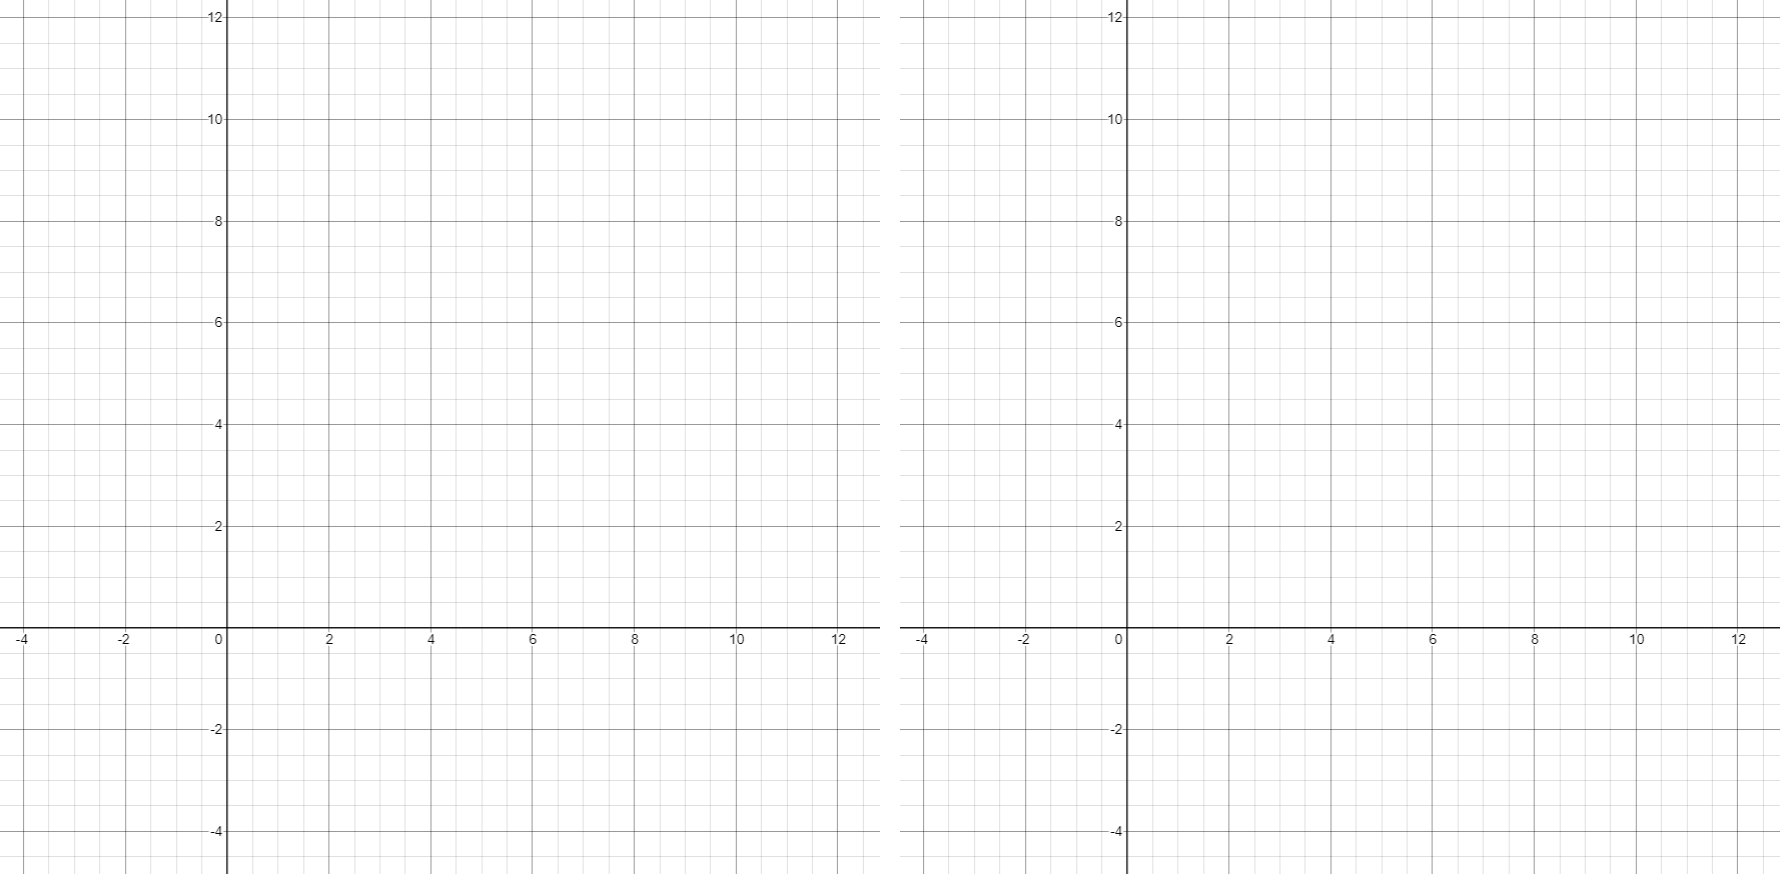
\includegraphics[width=1.1\linewidth]{empty-graphax2}
	
	\item Find the solution space and label corner points.
	\begin{multicols}{2}
		\begin{align*}
			6x+3y &\leq 24 \\
			3x + 6y &\leq 30 \\
			x,y &\geq 0
		\end{align*}
		\vfill\null
		\columnbreak
		\begin{tabular}{c|c}
			x & y \\ \hline
			0 &  \\
			& 0 \\ \hline
			0 &  \\
			& 0
		\end{tabular}
		\vfill\null
	\end{multicols}
	
	

%	\item Find the solution space and label corner points.
%		\begin{align*}
%			x+y &\leq 10 \\
%			5x+3y &\geq15 \\
%			-2x+3y &\leq 15 \\
%			2x - 5y &\leq 6
%		\end{align*}
%	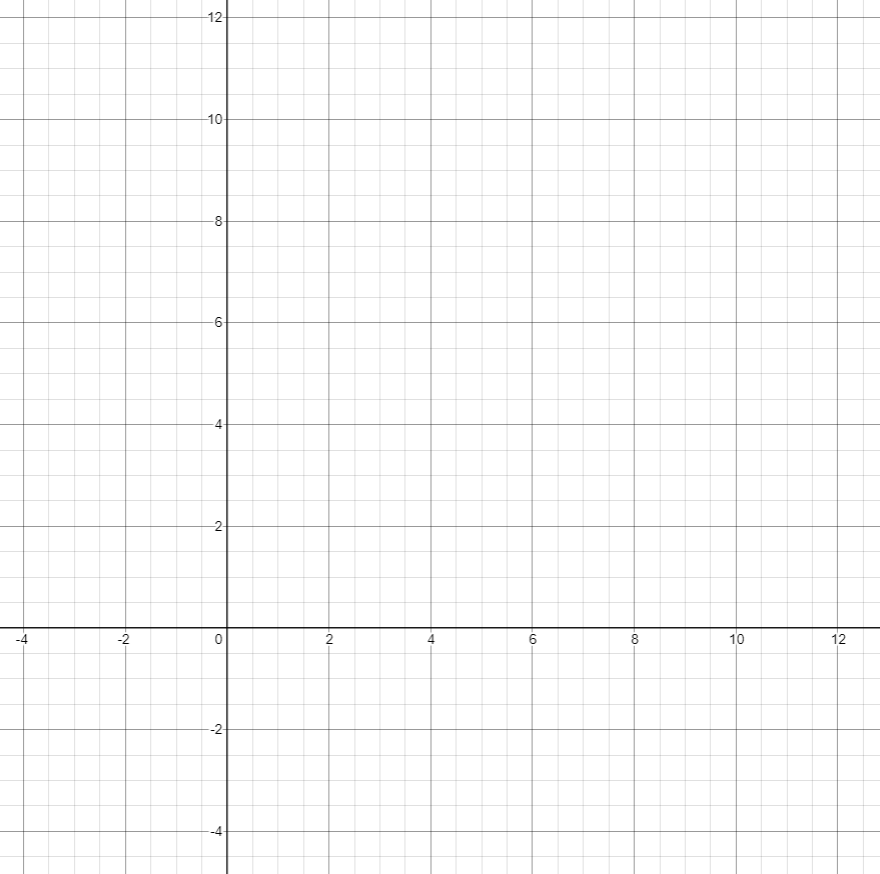
\includegraphics[width=0.8\linewidth]{empty-grapha}
	
	
\end{enumerate}

\cleardoublepage

\section{Linear Programming}
\begin{enumerate}
	\item Maximize and minimize
	\begin{multicols}{2}
		$$P = 6x +8y$$
		subject to 
		\begin{align*}
			x+y \leq 3 \\
			x+3y \leq 4 \\
			4x+5y \geq 20 \\
			x,y \geq 0
		\end{align*}
	
		\begin{tabular}{|c|c|}
			\hline
			Corner point & Objective value \\
			\hline
			(x,y) & $P=6x+8y$ \\
			\hline
			 &  \\
			\hline
			& \\
			\hline
			& \\
			\hline
			& \\
			\hline
			& \\
			\hline
			& \\
			\hline
		\end{tabular}
	\end{multicols}
	
	\hspace{-1.5cm}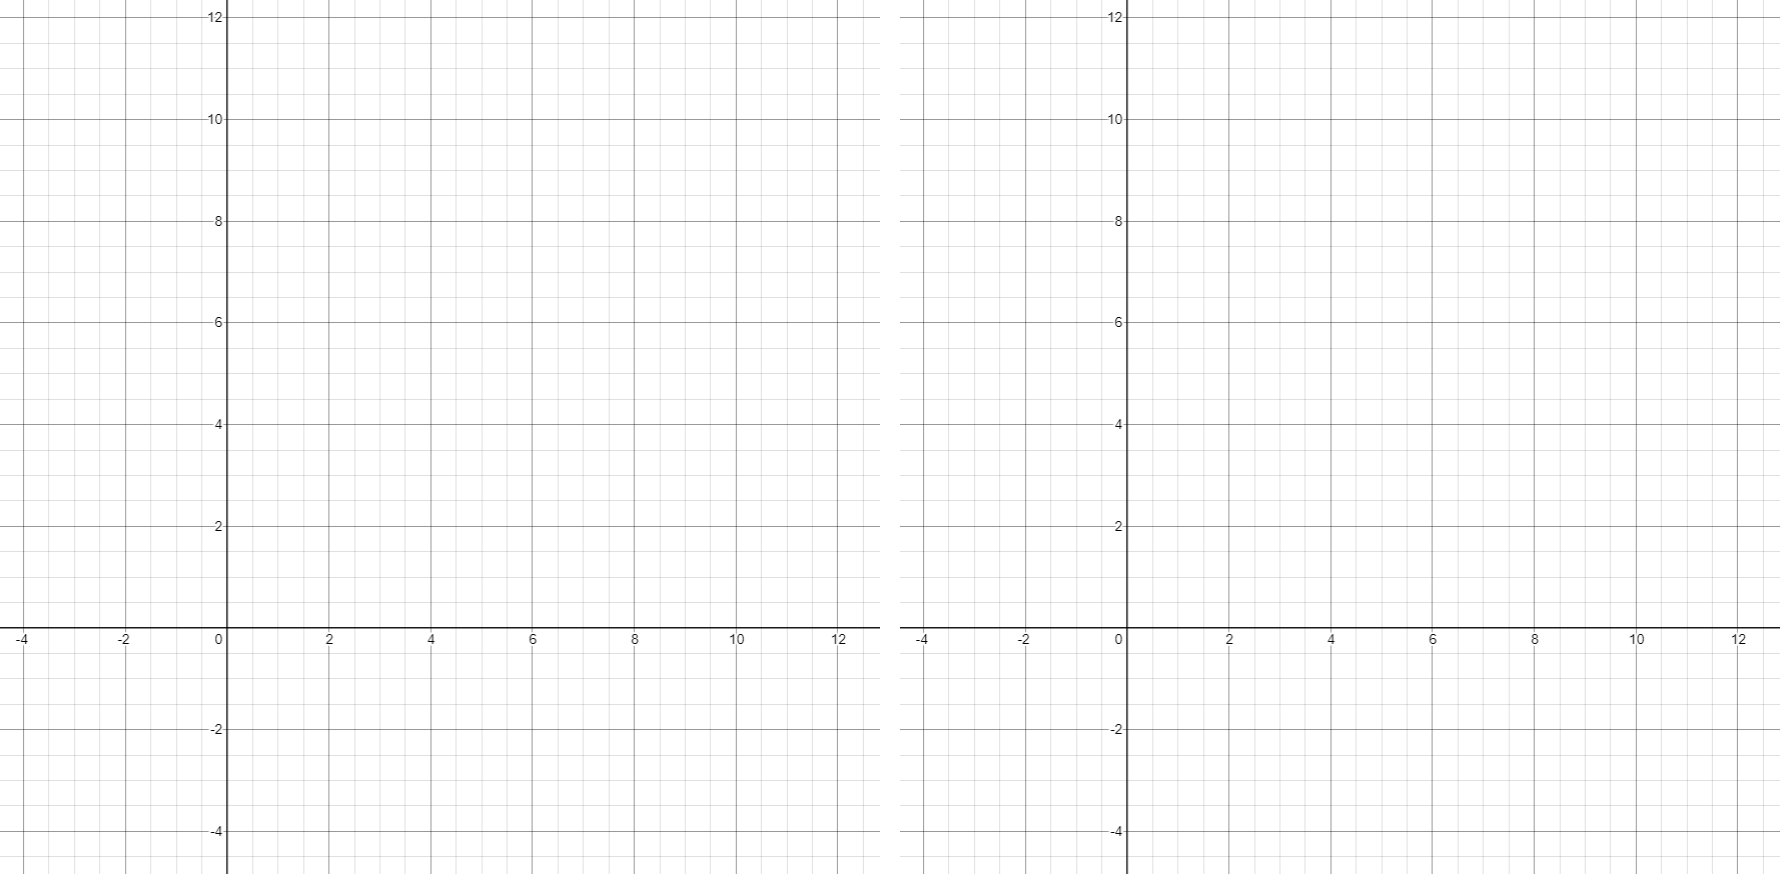
\includegraphics[width=1.1\linewidth]{empty-graphax2}
	
	
	\item Maximize and minimize
	\begin{multicols}{2}
		$$C = 8x +7y$$
		subject to 
		\begin{align*}
			4x+3y \geq 18 \\
			x+3y \geq 9 \\
			x,y \geq 0
		\end{align*}
	
	\begin{tabular}{|c|l|}
		\hline
		Corner point & Objective value \\
		\hline
		(x,y) & $C=$ \\
		\hline
		&  \\
		\hline
		& \\
		\hline
		& \\
		\hline
		& \\
		\hline
		& \\
		\hline
		& \\
		\hline
		\end{tabular}
	\end{multicols}
	

\cleardoublepage
	\item A fruit grower can use two types of fertilizer in  orange grove, brand A or brand B. The amounts (in pounds) of nitrogen, phosphoric acid, and chloride in a bag of each brand are given in the table. Tests indicate that the grove needs at least 2700 pounds of phosphoric acid and at most 500 pounds of chloride. (A) If the grower wants to maximize the amount of nitrogen added to the grove, how many bags of each mix should be used? and (B) If the grower wants to minimize the amount of nitrogen added to the grove, how many bags of each mix should be used?
	\\\\
	\begin{tabular}{|c|c|c|}
		\hline
		& \multicolumn{2}{c|}{Pounds per bag} \\
		\hline
		& Brand A & Brand B \\
		\hline
		Nitrogen & 5 & 7 \\
		\hline
		Phosphoric Acid & 6 & 6 \\
		\hline
		Chloride & 2 & 1 \\
		\hline
	\end{tabular}
	\\\\
	Write the Objective function and the problem constraints (inequalities) needed to solve this problem. Then solve graphically.
	\vspace{2.5cm}
	\\
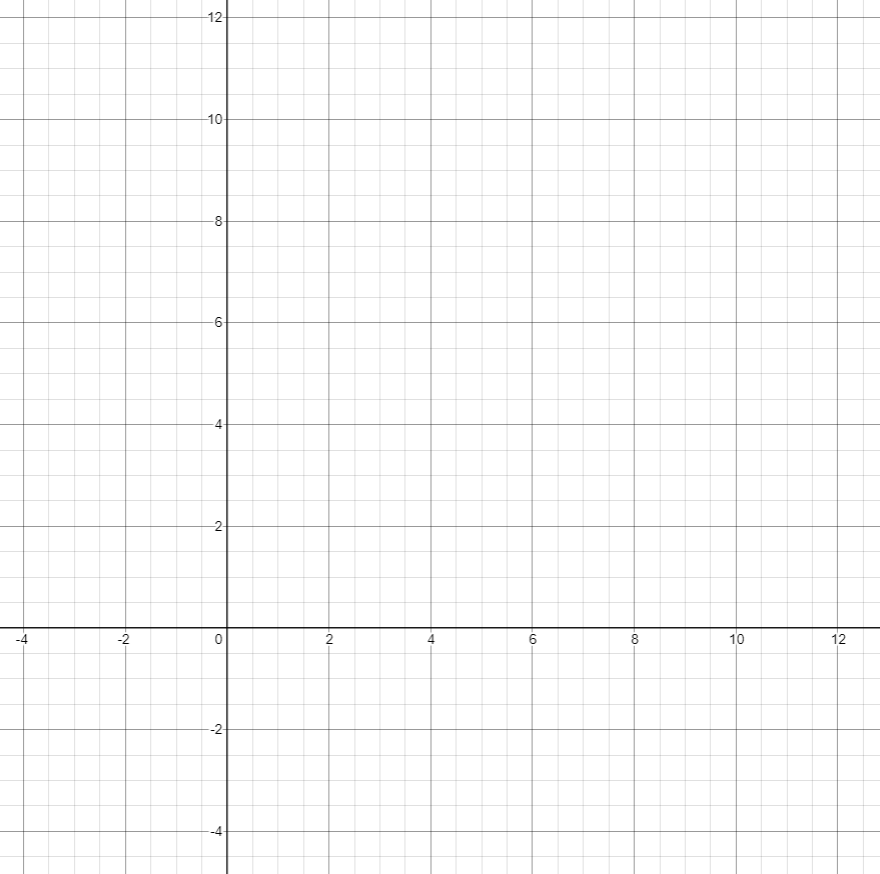
\includegraphics[width=0.7\linewidth]{empty-grapha}
	
\end{enumerate}


\cleardoublepage

\section{Sets}
	\begin{multicols}{3}[Find the resulting set]
		\begin{itemize}
			\item $\{1,2,3\} \cup \{4,8,16\}$
			\item  $\{1,2,3\} \cap \{4,8,16\}$ 
			\item  $\{3, 4, 5\} \cap \{4,8,16\}$ 
		\end{itemize}
	\end{multicols}
\vspace{2cm}
	\begin{multicols}{3}[True or false]
		\begin{itemize}
			\item $\{3,1\} \subseteq \{1,2,3,4\}$
			\item $1 \in \{4,8,16\}$ 
			\item $\{1,4\} = \{4\}$ 
		\end{itemize}
	\end{multicols}
\vspace{2cm}
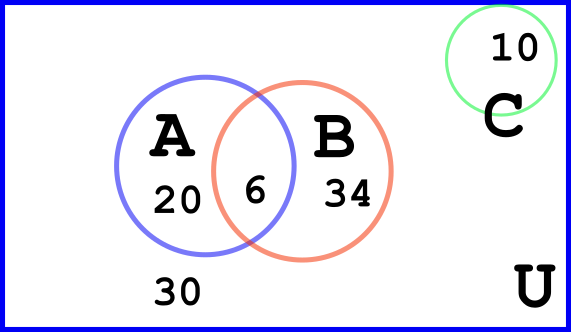
\includegraphics[width=0.8\linewidth]{venn-3}\\
	\begin{multicols}{3}[Determine the number of elements]
		\begin{itemize}
			\item $n(A)$
			\item $n(A\cap B)$ 
			\item $n(C')$
			\item $n(A\cap B')$
			\item $n(A\cup B)$ 
			\item $n((A\cup B)')$ 
		\end{itemize}
	\end{multicols}



\end{document}
